\chapter{Audio Data Hiding based on Dynamic Phase Coding}
This section presents an audio data hiding method that we used in our project. This method implements the technique of embedding watermarks into the phase spectrum of audio signal. To increase robustness, we choose low frequencies regions to do embedding because most of audio information is stored at those ranges. This method of phase modification causes sound distortion in proportion with the magnitude of frequencies components. Hence, we base on the magnitudes to determine how much change we want to apply to the original phase components. By this, we can balance inaudibility and robustness. We also held experiments with our method and the results show that our watermarked audio signal is inaudible.
\section{Introduction}
Audio data hiding methods generally should satisfy following standards: \textit{inaudibility, blindness, robustness,} and \textit{high capacity}. There are many trade offs amongs these requirements that make it very hard to achieve a perfect solution. To maintain \textit{inaudibility}, we should employ watermark embedding at perceptually insensitive features. But on the other hand, audio processing can distort the watermark without degrading the audio quality. Therefore, it is a very important task in our embedding method that we choose the appropriate acoustic features that satisfy both \textit{inaudibility}, and \textit{robustness}.

In our embedding method, we divide audio data into frames and embed information directly into the samples in the time domain or frequencies components in the transformed domain. As we mentioned earlier, there are a lot of watermark embedding techniques. We focus on the phase coding method and employ the technique of QIM into the processing of frequencies components. Our experimental results show that the watermark is robust but the audio quality is decreased when the bit rate increases. We modify the phases of frequencies component based on how strong they are. The bigger the frequency magnitude, the less we apply QIM into the phase, in order to reduce sound distortion. In other words, the amount of phase modification is adjusted according to the frequency's magnitude. Strong frequency components are more sensitive to the amount of change in the phase of that component. Therefore, larger magnitude frequency components have small phase modification and vice versa. This is where we achieve both low sound distortion as well as robustness, which means a balanced trade off between \textit{inaudibility}, and \textit{robustness.} 

\section {Proposed Method}
\subsection{Quantization index modulation}
\begin{figure}[bt]
\center
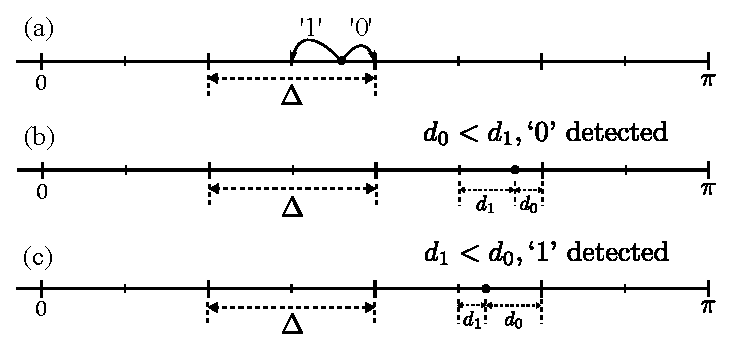
\includegraphics[width=.9\columnwidth]{QIMDemo_v1.eps}
\caption{Illustration of watermarking based on QIM: (a) embedding, (b) detection of `0', and (c) detection of `1'}
\label{fig:QIM}
\end{figure}
QIM has been considered as a class of provably good methods for digital watermarking \cite{qim}. The procedure of embedding and detecting watermarks is quite simple. Figure \ref{fig:QIM} shows an illustration of embedding and detection processes. To embed a bit $m$, `0' or `1' into a scalar variable $x$, we quantize $x$ to the nearest point that is an even or odd multiple of $\frac{\Delta}{2}$, respectively as (\ref{eq:QIMEncoder}). The obtained variable, $y$, is sent to receivers and might be affected by channel noise, hence becomes $\hat{y}$. To decode the embedded bit from $\hat{y}$, we calculate the distances between $\hat{y}$ and the nearest even multiple of $\frac{\Delta}{2}$, $d_0$ and the nearest odd multiple of $\frac{\Delta}{2}$, $d_1$ and then compare $d_0$ and $d_1$ to decode the bit as (\ref{eq:QIMDecoder1}) and (\ref{eq:QIMDecoder2}).

\label{eq:QIMEncoder}
\begin{align}
\label{eq:QIMEncoder}
y = Q(x,m) =
\begin{dcases} 
\Delta\left\lfloor\frac{x}{\Delta}+\frac{1}{2}\right\rfloor &\mbox{if } m = \mbox{`0'}\\ 
\Delta\left\lfloor\frac{x}{\Delta}\right\rfloor + \frac{\Delta}{2} &\mbox{if } m = \mbox{`1'}
\end{dcases}
\end{align}
where $\lfloor .\rfloor$ is the floor function and $\Delta$ is the QIM step size.
\begin{align}
\label{eq:QIMDecoder1}
d_j &= \hat{y} - Q(\hat{y},j), \quad j = \{\mbox{`0'},\mbox{`1'}\} \\
\label{eq:QIMDecoder2}
\hat{m} &= \arg\min_j d_j
\end{align}

\subsection {Principle of dynamic phase coding}
The original audio signal is processed by applying QIM to the phase spectrum. The result is a inaudible, robust, and reliable audio watermarking system with the following characteristics:
\begin{itemize}
\item{Phase modification is inaudible, that makes our embedded watermark is also inaudible}
\item{Most of audio information is distributed in low frequencies, thus this frequency region is more robust against attacks and should be chosen for embedding}
\item{Amount of change in the phase spectrum makes sound distortion in proportion with the magnitude spectrum of that frequency component. Therefore, we based on the magnitude to determine how much change we apply into the phase spectrum}
\item{Frequency components with extremely low magnitude are non-meaningful and very unreliable. So, we exclude those componens from our embedding process by establish a magnitude threshold.}

In the section, we investigate whether our method can help increase robustness while maintain the inaudibility by examine the above points.
\end{itemize}

\subsection{Watermark embedding}
We start off by spliting an original audio signal \(x(n)\) into many smaller frames \(x_i(n)\) with a fixed frame length. We also have a watermark string that is represented by binary bits \(s_i(l)\). We will employ the steps in Figure 4.2 to embedd \(s_i(l)\) into \(x_i(n)\).
\begin{itemize}
\item{\textbf{Step 1.}} Original frame \(x_i(n)\) is transformed into the Fourier spectrum \(X_i(\omega)\) by fast Fourier transform (FFT). Magnitude spectrum \(|X_i(\omega)|\) and phase spectrum \(\angle X_i(\omega)\)are calculated.
\item{\textbf{Step 2.}} We exclude the frequencies components whose magnitude are too small from the the embedding process. Specifically, we select the components whose magnitudes are larger than \(0.001\).

We then apply a dynamic phase coding system into our process. QIM step sizes are the amount of phase modification is determined based on its corresponding magnitude. First, magnitudes are normalize to 1 and linearly divided into \(L\) ranges in which each ranges has a corresponding step size. The higher the range, the smaller the step size.

Suppose that we have a set of \(L\) QIM step sizes, $\{\Delta_1, \Delta_2, ..., \Delta_L\}$, where $\Delta_1 > \Delta_2 > ... > \Delta_L$. The QIM step size for an embedding component $f$, namely $\Delta$, is determined as follows.

\begin{align}
%\nonumber |\hat{X}_i(f)| &= \frac{|X_i(f)|}{\max(|X_i(\omega)|)} \\
%\Delta &= \Delta_u, \mbox{where}\ u = \lceil L |\hat{X}_i(f)| \rceil
\nonumber |\hat{X}_i(f)| &= \frac{|X_i(f)|}{M} \\
\Delta &= \Delta_u,
\end{align}
 where $u = \lceil L |\hat{X}_i(f)| \rceil$ (if $u>L$, $u=L$) and $M$ is the parameter that represents for the maximum amplitude of most frequency components.

\item{\textbf{Step 3.}}  The bits $s_i(\ell)$ are encoded into the phase of the selected components by (\ref{eq:QIMEncoder}) and a quantized phase spectrum $\angle Y_i(\omega)$ is obtained. Although each bit can be embedded in only one component, it is embedded in several components to increase robustness. The bit rate is adjusted by changing the number of components for each bit.

\item{\textbf{Step 4.}} The magnitude spectrum, $|X_i(\omega)|$ and the quantized phase spectrum, $\angle Y_i(\omega)$, are combined into Fourier spectrum $Y_i(\omega)$ which is then transformed into time domain signal \(y_i(n)\) by inverse Fourier transform (IFFT).

Finally, all the processed frames are combined together to yield a watermarked signal \(y_n()\).

\end{itemize}

\begin{figure}[tp]
\center
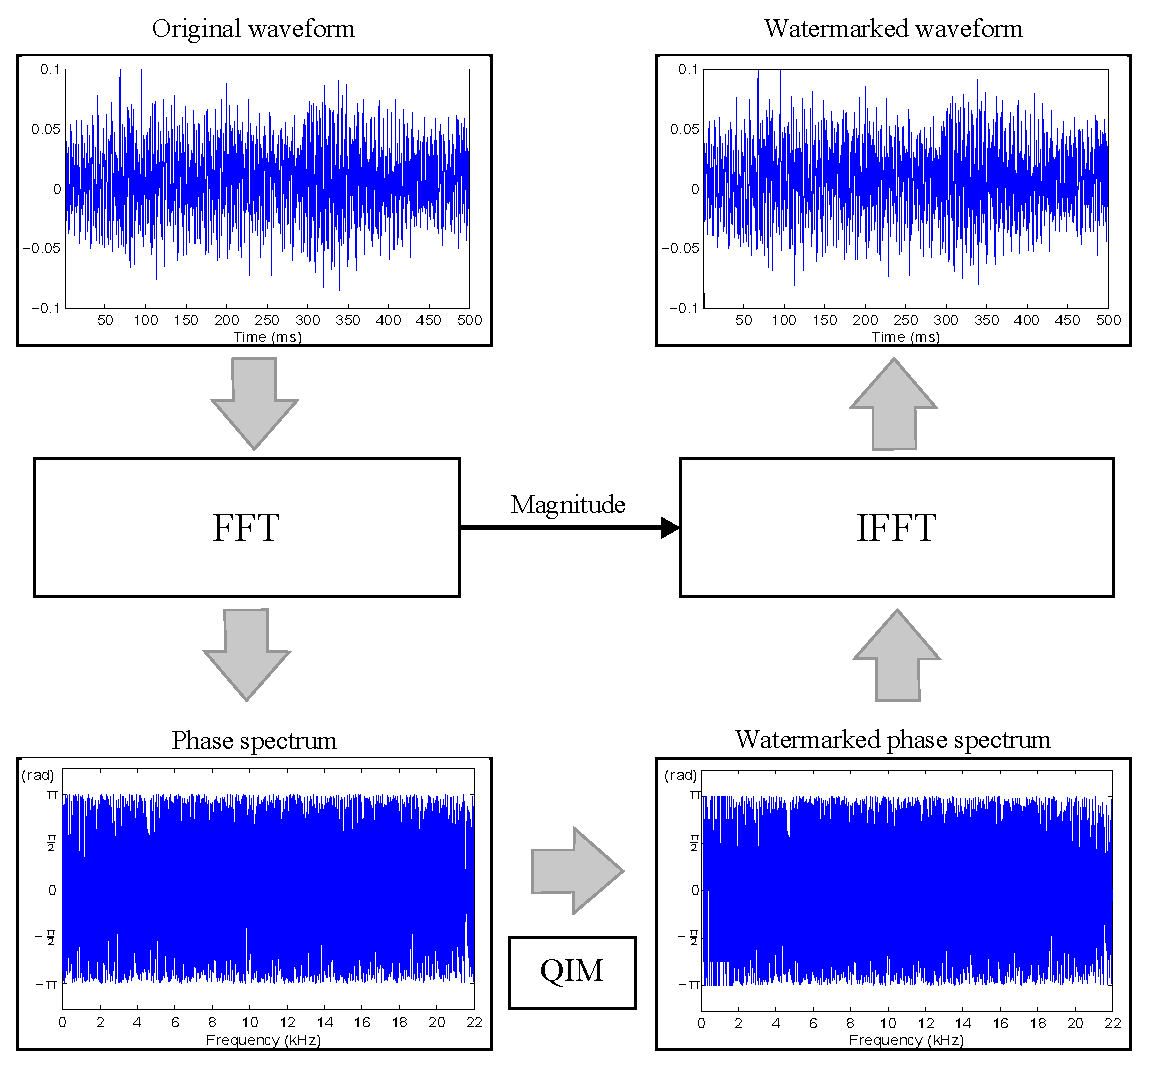
\includegraphics[width=1\columnwidth]{Illustrative_Example.eps}
\vspace{0mm}
\caption{Process of watermark embedding: conversion of a frame of time-domain samples into the Fourier domain, QIM watermark addition, and conversion back to the time-domain.
}
\label{fig:QIMWM_illustrative}
\vspace{0mm}
\end{figure}
\vspace{0mm}

% --------------------------------------------------------------------------

\begin{figure}[tp]
\center
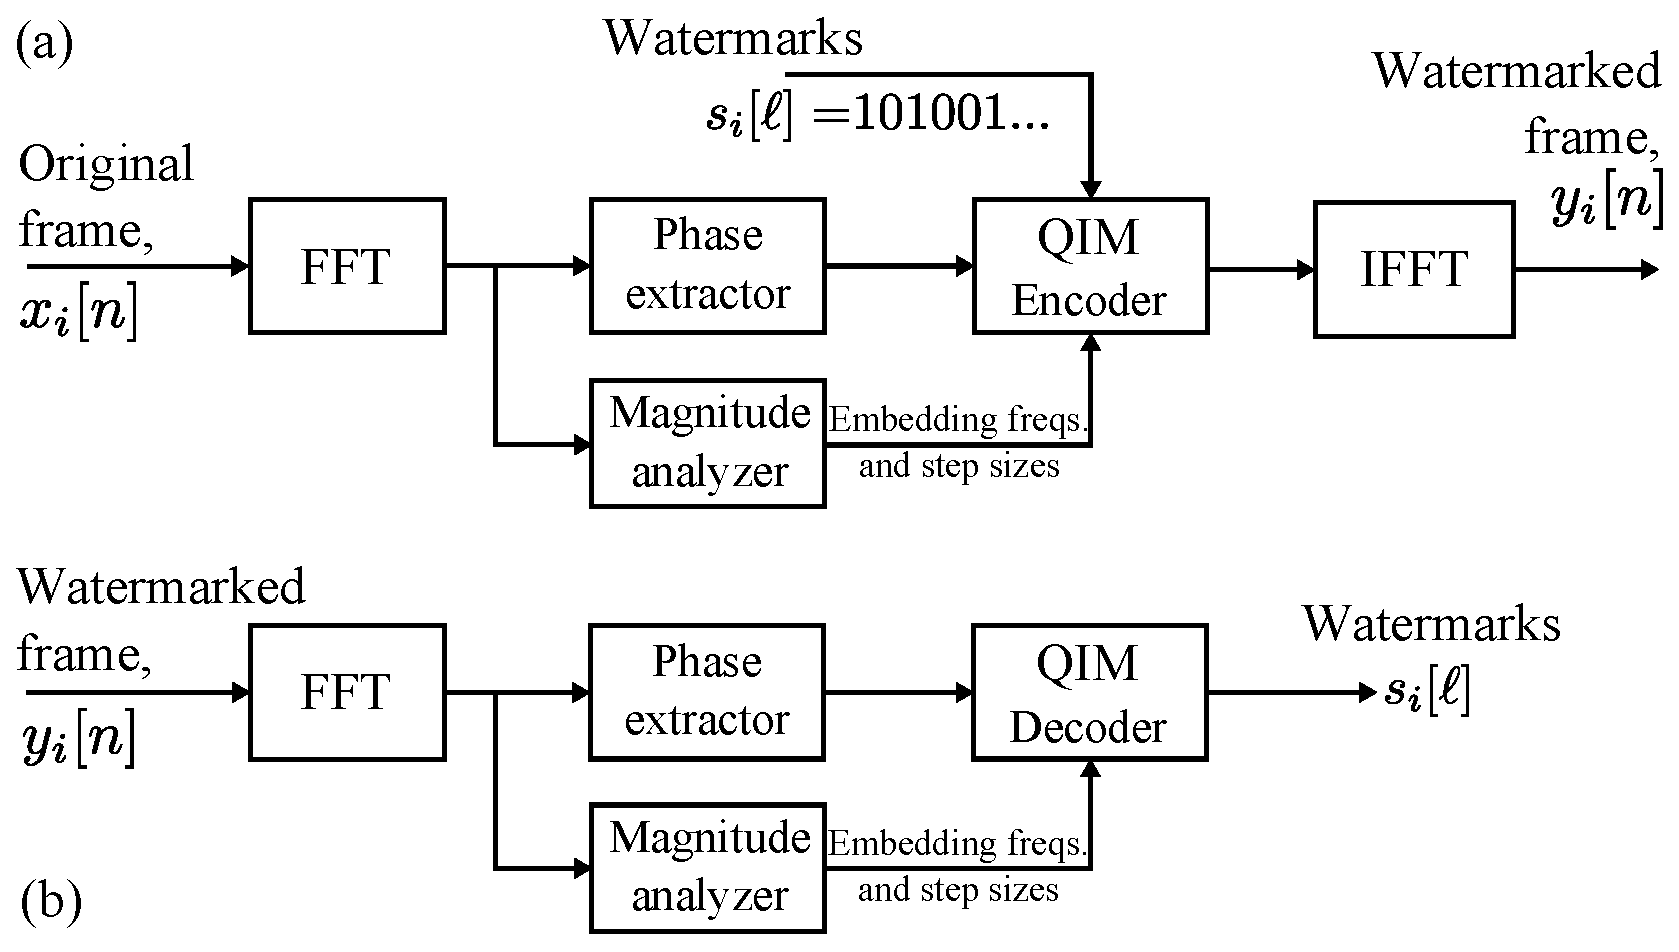
\includegraphics[width=1\columnwidth]{ProposedScheme.eps}
\caption{Proposed scheme of audio watermarking: (a) embedding process and (b) detection process}
\label{fig:WMScheme}
\end{figure}

\subsection{Watermark detection}
The detection process also starts with frame segmentation of the watermarked signal, \(y(n)\) into frames \(y_i(n)\) with the same frame size as in the embedding process. Figure \ref{fig:WMScheme}(b) shows a block diagram of the process that detects watermark bits from a watermarked frame involving three steps as follows.

\textbf{Step 1.} Watermarked frame \(y_i(n)\) is firstly transformed into $Y_i(\omega)$ by FFT. Phase spectrum $\angle Y_i(\omega)$ is calculated.

\textbf{Step 2.} The embedding frequency components and corresponding QIM step sizes are determined as in Step 2 in the embedding process.

\textbf{Step 3.} The embedding components are decoded by (\ref{eq:QIMDecoder2}) to extract all the bits. The output bits, $s_i(\ell)$, are determined by majority decision, e.g., if the number of `0', $N_0$, are greater the number of `1', $N_1$, the output is `0'.

These steps are repeated until we reach the final frame.
% -------------------------------------------------------------------------

\section{Evaluations}
\subsection{Parameters}
Before demonstrate our experiment, we would introduce many constant used in our entire project, including this experiment. Our system depends on many parameters in the process of watermark embedding. As we mentioned earlier, it is difficult to achieve an ideal settings when we have many dimensions. For instance, keeping the error rate low enough to not produce an incomplete watermarking, or else it would affect greatly on the user experience. At the same time, we also have to maintain a reasonable amount of embedding space to satisfy the embedding need. Those two are the biggest trade-offs of our system. It then becomes very important to experiement with different settings to come up with a optimal solution for our specific problem. There are two parameter that we need to keep eyes on.

\begin{table}
\centering
\caption{Configuration on the QIM step sizes with regard to the normalized magnitude}
\vspace{2mm}
\addtolength{\tabcolsep}{-6pt}
\begin{tabular}{|m{3cm}|m{2.25cm} | m{2.25cm} | m{2.25cm} | m{2.25cm} | m{2.25cm} m{0cm}|}
 \hline 
& \multicolumn{5}{c}{QIM step sizes ($\Delta$)} & \\ [.2cm]
\hline
Normalized magnitude & (0, 0.2] & (0.2, 0.4] & (0.4, 0.6] & (0.6, 0.8] & (0.8, 1] & \\
\hline
Set 1 & $\tfrac{\pi}{2}$ & $\frac{\pi}{4}$ & $\frac{\pi}{6}$ & $\frac{\pi}{8}$ & $\frac{\pi}{10}$ & \\ [.2cm]
\hline
Set 2 & $\tfrac{\pi}{3}$ & $\frac{\pi}{5}$ & $\frac{\pi}{7}$ & $\frac{\pi}{9}$ & $\frac{\pi}{11}$ & \\ [.2cm]
\hline
Set 3 & $\tfrac{\pi}{4}$ & $\frac{\pi}{6}$ & $\frac{\pi}{8}$ & $\frac{\pi}{10}$ & $\frac{\pi}{12}$ & \\ [.2cm]
\hline
\end{tabular}
\addtolength{\tabcolsep}{6pt}
\label{tab:QIMStep}
\end{table}

\subsubsection{QIM step sizes}First, as we employ the teachnique of dynamic phase coding, we depend on the magnitude of frequency coponents to determine the appropriate phase change. Specifically, we divide our frequency range into \(5\) small part, each with its own setting called step sizes. This number step size is very important to embedd into the phase component of the frequency. If we apply too much shift into the phase components, the audio quaility would decrease. Otherwise, too subtle change could not be successfully decoded. To figure out the best settings, we have to set up several experiments with different ranges of step sizes and record the resulting audio quality as well as the correctness percentage. The QIM step sizes are chosen as integer divisions of \(\pi\)
to reduce wrapping errors. We investigated the proposed method with three sets of five
QIM step sizes as shown in Table \ref{tab:QIMStep}.
\subsubsection{Embedding space}
We want to measure how many bits we have in 1 second for our watermark embedding to be effective while still satisfy acceptable capacity. In audio processing, we normally use a sampling frequency of \(44.1kHz\). Audio data is splitted into frames with a fixed frame length of \(22050\). While the audio data is stored in \(16\) bit integers. We have our sampling frequency equals \(44.1kHz\), which means there are \(44100\) integers of audio data in \(1\) second. Hence, if we choose our frame length equals \(22050\), each frame would be \(0.5\) second and bits per second is twice bits per frame \((BpS=2BpF)\). 

In the process of transforming audio data in time domain to the frequency domain, we can choose the range to apply the transformation. At this stage, we can either transform the whole audio file at once or split into smaller frames with fixed length. If we put the whole file into Fourier Transform at once, the frequencies along the files would be mixed together, produce an array of frequencies components from small to big frequency. Numerous components with the same frequencies would be merge into one as our transformation result. Clearly, this approach does not efficient in terms of computation and physics. On one hand, it adds memory overhead as we need to store the enormous transformation result the whole time, while we only need to store a much smaller amount if we split the file into frames. Moreover, mixing frequencies components into only \(1\) component and apply modification would result in the change in all the frequencies components corresponding to that frequency, and of couse this would harm both our audio quality and embedding correctness. Hence, we chose the second approach, spliting audio data into frames with fixed length. However, this result leads us to another question that, what is the resonable length for a frame? 
According to the Nyquist-Shannon sampling theorem, which states that, for a given sample rate \(f_s\), perfect reconstruction is guaranteed possible for a bandlimit \(B<\frac{f_s}{2}\). Plus, recall that the common maximum frequency that human ear can percept is approximately \(20kHz\). Which means, to effectively sample our audio data, we should choose the sample rate \(f_s>40kHz\). It is common in the field of audio processing that we choose \(f_s=44100Hz\) and frame length \(FL=\frac{f_s}{2}=22050\). 

In order to decrease the possibility of embedding into unstable frequencies components, which usually located at frequencies higher than \(1600Hz\). In fact, this low frequency region is where most of the sound content lies. Therefore, from the property of discrete Fourier transform, the bin corresponding to \(1600Hz\) frequency is at the \(\frac{FL}{f_s}1600=800^{th}\) bin. Hence, we only have \(800\) frequency bins to do embedding.

Next, we look closer into the \(800\) bins we got. To further increase our correctness, we repeat each bit consecutively many times. In particular, we chose \(BITREPEAT=5\), if we have \(1\) bit is incorrectly decoded, we still have \(4\) other bits to rely on. This greatly increase our embedding correctness. As we chose \(BITREPEAT=5\), we only have \(\frac{800}{5}=160\) bits left. But \(8\) bits form a character, which left us \(20\) characters per frame. 
\subsubsection{Summary}
In summary, we have the following parameters
\begin{itemize}
\item{\textbf{Step sizes}} We use 3 arrays of step sizes as described in Table \ref{tab:QIMStep}
\item{\textbf{Maximum number of embedding samples per frame}} \(SpF=800\)
\item{\textbf{Maximum number of embedding bits per frame}} \(BpF=160\)
\item{\textbf{Maximum number of embedding bits per second}} \(BpS=320\)
\item{\textbf{Maxium number of embedding characters per second}} Character per second \(CpS=40\)
\item{\textbf{Bit repeats}} Number of times repeat a bit to ensure embedding correctness \(BitRepeat=5\)
\item{\textbf{Minumum frequency magnitude for embedding}} \(MagnitudeThreshold=0.001\)
\end{itemize}
\subsection{Experiment metrics}
\subsubsection*{Audio quality}
Inaudibility is tested by PEAQ which rates sound quality by the ODG from −4 (very annoying) to 0 (imperceptible).
\subsubsection*{Embedding correctness}
Bit detection rate is measured by BDR, the ratio between the numbers of correct bits and total bits.

Character detection rate is measured by CDR, the ratio between the number of correct characters and total characters.
\subsection{Effectiveness of proposed method}
The result of our test is shown as below. Relate from \ref{tab:QIMStep}, because of bigger phase modification, the first setting show better perfomance in terms of BDR and CDR, which are both at 99.97\%. The details of result is shown in Table \ref{tab:bdrcdr}.
\begin{figure}
\begin{center}
\begin{tabular}{ |c|c|c| } 
 \hline
  			& BDR & CDR \\ 
 Settings 1 &  99.97\% & 99.97\% \\ 
 Settings 2 &  99.96\% & 99.92\% \\ 
 Settings 3 &  99.93\% & 99.87\% \\ 
 \hline
\end{tabular}
\end{center}
\caption{BDR and CDR test result}
\label{tab:bdrcdr}
\end{figure}

\begin{figure}[h]
	\centering
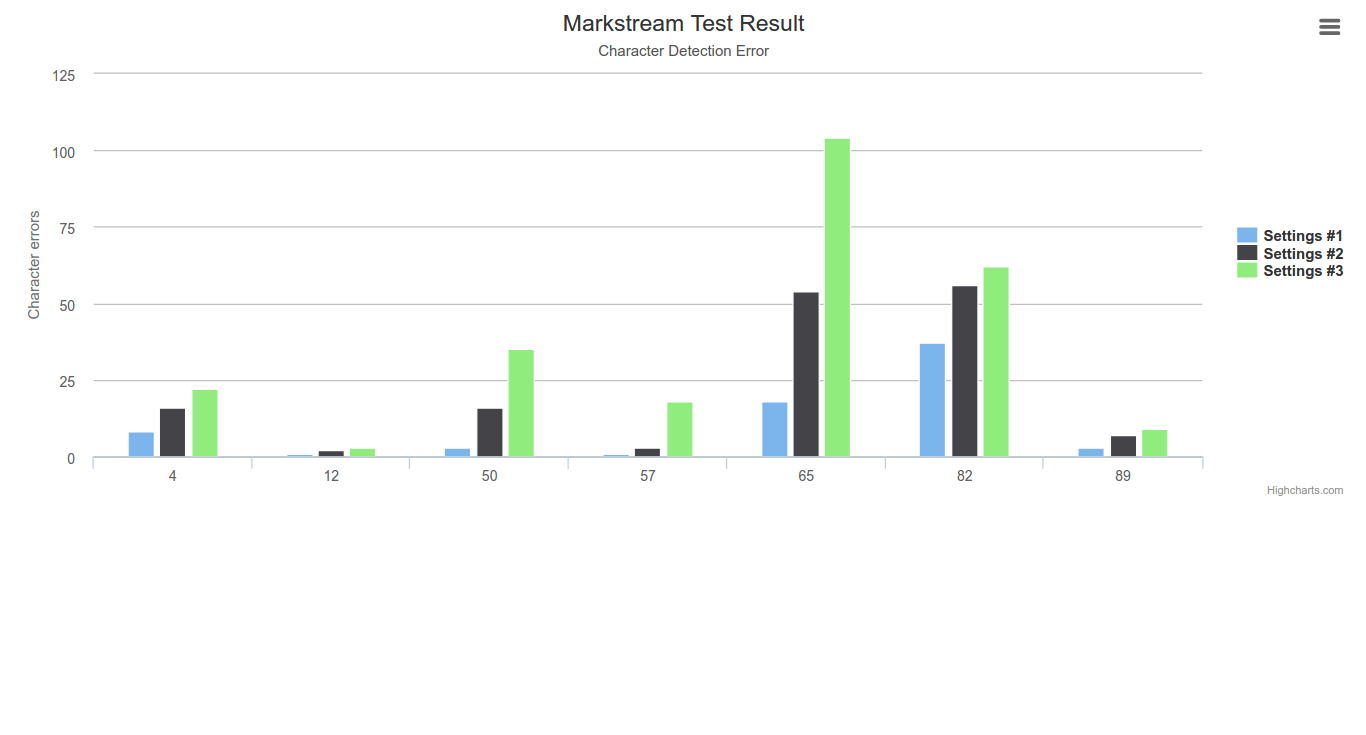
\includegraphics[width=\textwidth]{cdrmarkstream}
 	\caption{Character detection rate test result.}
 	\label{fig:CDRMarkstream}
\end{figure}

\section{Summary}
We proposed an audio watermarking method based on dynamic phase coding. Watermarks are embedded into low frequency components and the amount of change is determined based on the magnitude spectrum to balance inaudibility and robustness. We also employ 2 experiments to value the effectiveness of our proposed method. Our experiment had been carried to confirm the effectiveness of the DPC scheme.

The experimental results suggest that the proposed DPC scheme is more effective
than the SPC scheme, resulting in a better trade-off among the properties.
The proposed method is capable of embedding watermarks into audio signals at a
bit rate of 320 bits per second with the highest accuracy of watermark detection of 98\%. It has been re-vealed that the proposed method could satisfy the requirements of inaudibility, blindness, high capacity, and high reliability. 